\chapter{Implementierung}
\label{chap:implementation}

Auf Basis der entwickelten Konzeption folgt in diesem Kapitel die praktische Umsetzung.
Dabei werden die einzelnen Komponenten des Systems beschrieben und ihre Implementierung erläutert.
Neben technischen Aspekten wie der Strukturierung von Backend und Frontend sowie der Integration des Gutenberg-Editors wird auch auf die Realisierung der funktionalen Anforderungen eingegangen.

\section{Entwicklungsumgebung und Tools}

Für die Umsetzung des Projekts wurden verschiedene Tools eingesetzt.
Als Entwicklungsumgebung kam PHPStorm zum Einsatz, ergänzt durch PHPCS zur Einhaltung der WordPress-Codestandards.
Google Chrome diente als Browser, während die lokale Entwicklung mit Local WP eingerichtet wurde.
Zur Verwaltung von Paketen und Abhängigkeiten wurde npm verwendet und die Versionierung des Projekts erfolgte über GitHub.

\subsection{Projektsetup}

Im ersten Schritt der Implementierung wurde eine lokale Entwicklungsumgebung mittels Local WP eingerichtet.
Die Entwicklungsumgebung basiert auf einem nginx-Webserver mit PHP Version 8.4.10 und einer MySQL-Datenbank in Version 8.0.35.
WordPress wurde in der Version 6.8.2 installiert und mit den Standardkonfigurationen eingesetzt.
Es wurden keine zusätzlichen Anpassungen an der Grundkonfiguration vorgenommen und keine weiteren Plugins hinzugefügt, um eine möglichst neutrale Ausgangsbasis für die Umsetzung zu gewährleisten.
Zwecks Versionierung wurde Git auf der GitHub-Instanz der elancer-team GmbH verwendet und ein neuer Branch im bestehenden Repository angelegt.
Der bestehende Stand des Plugins wurde abschließend in WordPress importiert und die eigentliche Implementierung begonnen.

\section{Plugin-Struktur und Architektur}

\subsection{Ausgangsbasis und Bereinigung}

Als Ausgangsbasis für die Implementierung wurde die WordPress Plugin Vorlage von DevinVinson\footnote{\url{https://github.com/DevinVinson/WordPress-Plugin-Boilerplate}} verwendet.
Diese Vorlage bietet eine standardisierte Struktur für WordPress-Plugins und folgt den offiziellen WordPress-Entwicklungsrichtlinien im Hinblick auf die Best Practices~\cite{wordpress2025BSP}.

Im ersten Schritt wurden die zuvor importierten Daten aus dem bestehenden Plugin-Stand in die Vorlage eingesetzt und eine umfassende Bereinigung durchgeführt.
Dabei wurden nicht verwendete Dateien identifiziert und entfernt.
Zu diesen Altlasten zählten diverse Assets und Abhängigkeiten, die bereits zum Zeitpunkt des Transfers keine Funktion mehr erfüllten oder redundant wurden.
\subsection{Migration und Anpassung der Komponenten}
\textbf{Migration zu Carbon Fields}

Nachdem die grundlegende Bereinigung der Daten abgeschlossen war, wurde mit der Migration von ACF Pro zu \gls{carbonfields} begonnen.
Wie in Kapitel \ref{chap:concept} konzipiert wurde Carbon Fields als Ersatz für ACF Pro implementiert.
Hierzu wurde eine dedizierte Klasse für den Boot-Prozess von \gls{carbonfields} erstellt und über Composer als Abhängigkeit in die neue Projektstruktur eingebunden.
Die Initialisierung erfolgt über einen Klassenaufruf, der das Framework zentral verfügbar macht, welche in Abbildung \ref{fig:carbon-fields-init} veranschaulicht ist.

\begin{figure}[H]
    \centering
    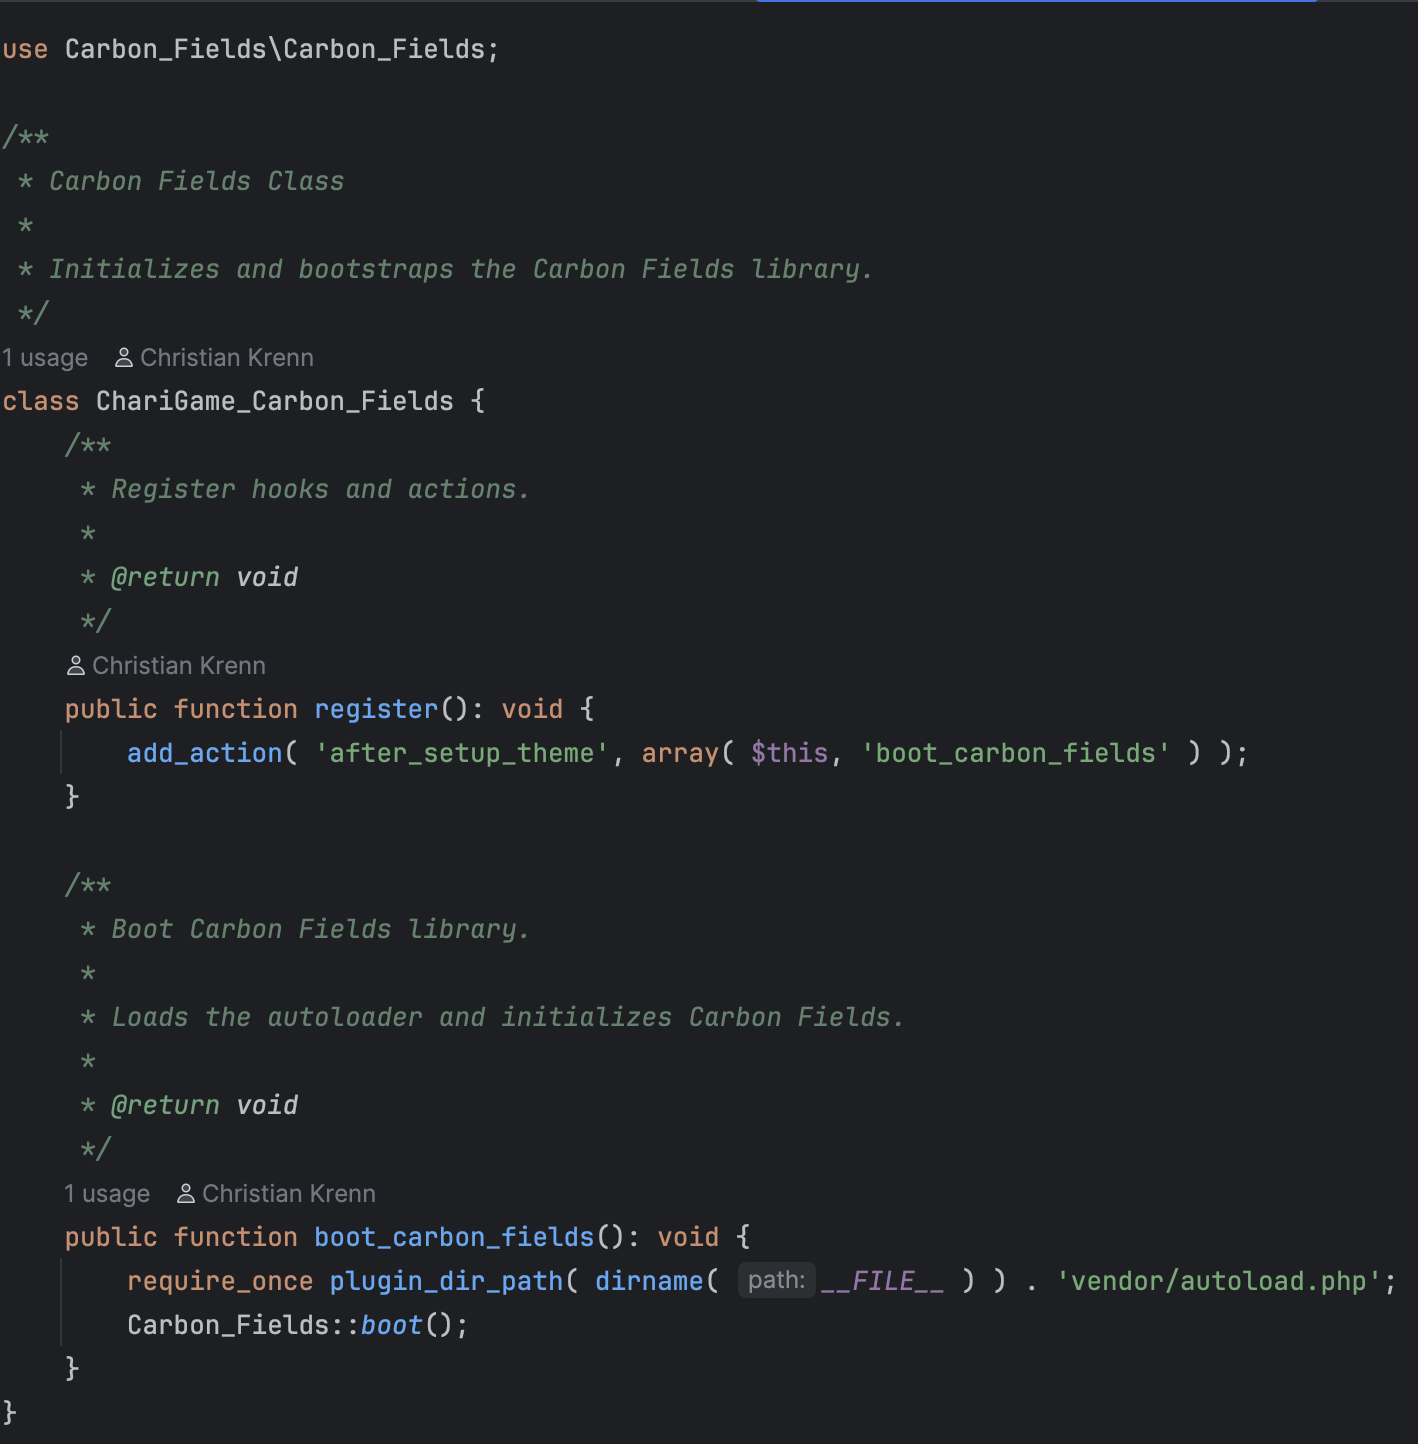
\includegraphics[width=1\textwidth]{images/carbon_fields_init}
    \caption{Aufbau der Klasse Charigame\_Carbon\_Fields (eigene Darstellung)}
    \label{fig:carbon-fields-init}
\end{figure}

Alle bestehenden \texttt{get\_field()}-Aufrufe des ursprünglich verwendeten ACF Plugins wurden daraufhin systematisch identifiziert und durch das entsprechende \gls{carbonfields}-Pendant ersetzt.
Diese Migration gewährleistet die Kompatibilität mit der neuen Architektur und eliminiert die externe Abhängigkeit von ACF Pro vollständig.
Im Zuge der Migration der carbon\_get\_post\_meta() Aufrufe mussten im nächsten Schritt die verwendeten Custom Post Types auf die neu eingesetzte Carbon Field Struktur angepasst werden.
\\\\
\textbf{Custom Post Types und REST API}

Alle Custom Post Types wurden neu aufgebaut, um einen einheitlichen Duktus innerhalb des \textit{ChariGame}-Plugins zu realisieren und die Funktionalität mit Carbon Fields zu gewährleisten.
Hier wurden die Namespace-Bezeichnungen angepasst und Klassen- sowie Datenbankbezeichnungen vereinheitlicht.
Darüber hinaus sind die Felder, welche dem Redakteur im Backend zur Verfügung gestellt werden, durch Carbon Fields ersetzt worden.
Die Ausführung des Custom Post Types der Recipients ist in Abbildung~\ref{fig:new-recipients-frontend} visualisiert.

\begin{figure}[H]
    \centering
    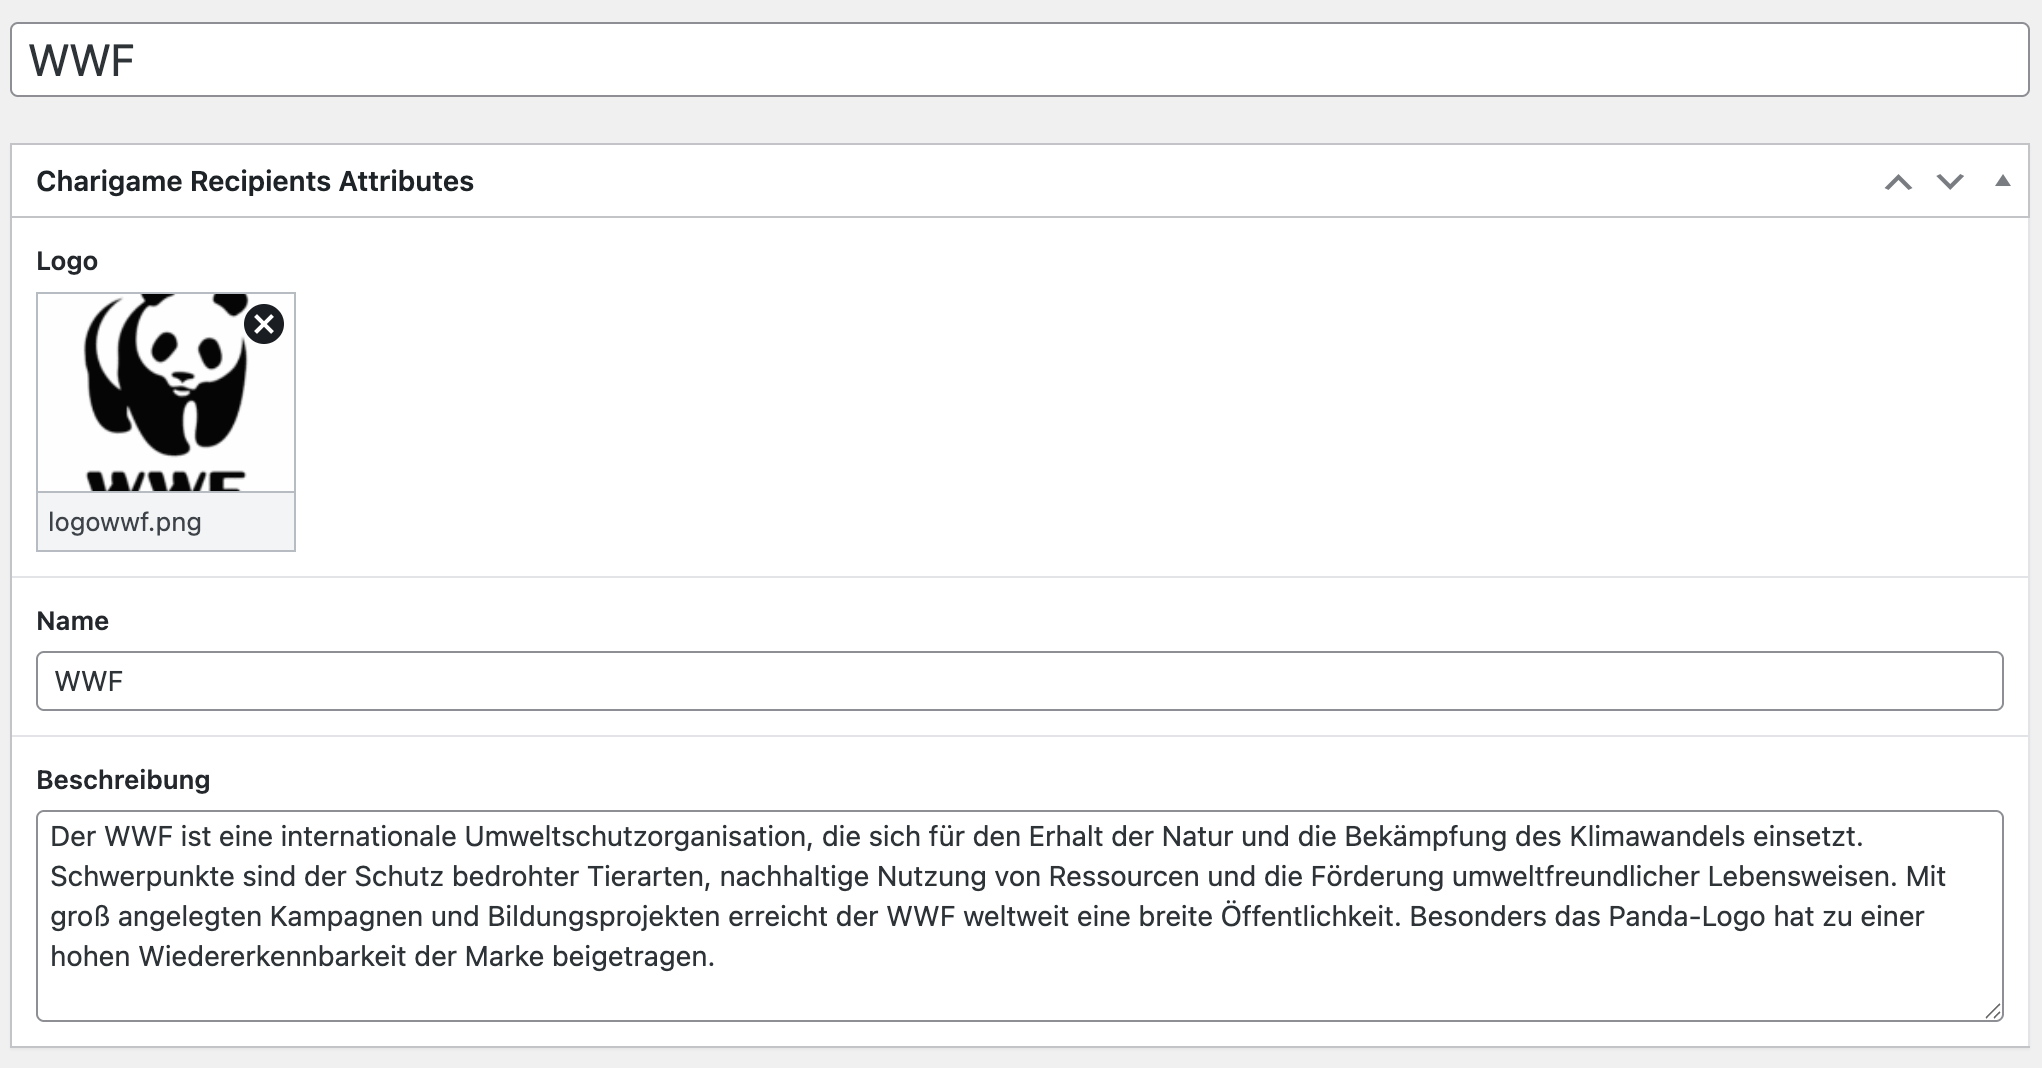
\includegraphics[width=1\textwidth]{images/new_recipients_backend}
    \caption{Recipients Frontend (eigene Darstellung)}
    \label{fig:new-recipients-frontend}
\end{figure}

Bei der Neudefinition der CPTs wurden wichtige Eigenschaften der Carbon Fields für die REST API freigegeben, um diese im Backend-Editor über React abrufen zu können.
Dies ist für die Umsetzung der Gutenberg-Blöcke und deren dynamische Eigenschaften erforderlich, da diese auf Kampagnendaten und verknüpfte Inhalte zugreifen.
Dazu wurden unter anderem Daten zu \texttt{game\_type}, \texttt{game\_settings}, \texttt{linked\_landing\_page} und \texttt{recipients} innerhalb der internen REST-Schnittstelle unter wp-json verfügbar gemacht.
\\\\
\textbf{Verzeichnisstruktur und Design-System}

Die Verzeichnisstruktur wurde anhand der Plugin-Vorlage von DevinVinson erweitert und modular aufgebaut.
Der Aufbau besteht aus verschiedenen Verzeichnissen, wobei die wichtigsten Verzeichnisse folgend kurz erläutert werden:

\begin{itemize}
    \item \textbf{includes/}: Kernfunktionalitäten und Klassen
    \item \textbf{admin/}: Backend-spezifische Komponenten, shadcn/ui-Styles
    \item \textbf{frontend/}: Frontend-Darstellung und Templates
    \item \textbf{blocks/}: Gutenberg-Block-Definitionen
    \item \textbf{assets/}: Statische Ressourcen (CSS, JS, Bilder, Icons)
    \item \textbf{src/}: Quellcode der Block-Entwicklung und Spiele
    \item \textbf{templates/}: Template-Dateien für die Darstellung
\end{itemize}
\vspace{0.5em}
\textbf{Design-System}

Für das Design im Front- und Backend wurde TailwindCSS verwendet.
Hierzu wurden zwei unabhängig voneinander bestehende CSS-Konfiguration erstellt.

Die erste Konfiguration erfasst alle Tailwind-Klassen aus dem gesamten Projektkontext und generiert diese sowohl für das Frontend als auch das Backend.
Die zweite Konfiguration ist spezifisch auf den Administrationsbereich und im speziellen auf die shadcn/ui Komponenten abgestimmt.

Diese Implementierung im Administrationsbereich nutzt die folgenden Bausteine:
\begin{itemize}
\item Eine PHP-portierte shadcn/ui-Bibliothek
\item Einen shadcn-Prefix zur Vermeidung von Konflikten mit WordPress-Styles
\item Vorgebaute CSS-Dateien im Verzeichnis admin/css/
\item Selektives Laden der Styles ausschließlich auf ChariGame-Admin-Seiten
\end{itemize}
Diese Trennung gewährleistet, dass sich die unterschiedlichen Styling-Systeme nicht gegenseitig beeinträchtigen und eine saubere Kapselung der Admin-Oberfläche ermöglicht wird.
\\\\
\textbf{Asset Manager und Template Loader}

Ein Asset Manager wurde implementiert, der selektiv die passenden Assets für Admin- und Frontendbereich lädt.
Im Admin-Bereich werden die zuvor erwähnten shadcn/Tailwind-Styles aus dem Design-System geladen.
Im Frontend bindet der Asset Manager die Game-Styles/-Skripte ein und bindet die Daten auf den vom \textit{Charigame} Plugin erstellten Seiten ein.

Der Template Loader stellt wiederrum sicher, dass Campaign-Inhalte das korrekte Template beziehen.
Für den Custom Post Type der Landingpages wurde festgelegt, dass diese nicht eigenständig betrachtet werden, sondern den Content ausschließlich in den Campaign-Templates ausgeben.
In diesem Fall führt der Template Loader Redirects auf die referenzierte Kampagne durch.
\\\\
\textbf{Login-System und Sicherheit}

Die Login-Logik wurde aus dem Frontend separiert und in einen dedizierten Login Manager überführt.
Das System implementiert mehrere Sicherheitsmaßnahmen, die im Kapitel~\ref{chap:concept} beschrieben wurden, darunter:

\begin{itemize}
    \item \textbf{\gls{nonce}-Validierung}: \texttt{wp\_verify\_nonce()} schützt AJAX-Endpoints
    \item \textbf{Input-Sanitizing}: \texttt{sanitize\_text\_field()}, \texttt{intval()} für Benutzereingaben
    \item \textbf{Session-Management}: Sessions werden früh gestartet und konsistent genutzt
    \item \textbf{Caching}: Datenbank- und User-Lookups werden im \gls{objectcache} gepuffert
\end{itemize}

Darüber hinaus wurde ein \gls{shortcode} erstellt, der den Content der Landingpages überträgt und diesen in die Campaign-Templates einsetzt.
Dies ermöglicht eine flexible Wiederverwendung der Landingpage-Inhalte und bildet eine stabile Möglichkeit die Inhalte auf der Campaign Seite nach erfolgreichem Login zu erzeugen.
\\\\
\textbf{Color Manager}

Der Color Manager verwaltet Kampagnenfarben und stellt diese systemweit zur Verfügung.
Die Implementierung erfolgt als Singleton-Klasse, damit sichergestellt wird, dass nur eine einzige Instanz des Managers bestehen kann.
Hier werden folgende Funktionalitäten bereitgestellt:

\begin{itemize}
    \item Automatische Kampagnen-Erkennung über URL-Kontext zwecks Zuordnung der Kampagnenfarben
    \item CSS-Variablen für den Frontend- und Adminbereich (\texttt{--color-primary}, etc.)
    \item JavaScript-Objekt \texttt{charigameColors} für den Block-Editor
    \item Fallback auf Standard-Farbpalette
\end{itemize}

\subsection{Backend-Integration und Dashboard}

Das bestehende Dashboard wurde vollständig überarbeitet und mit den shadcn/UI-Komponenten des neuen Design-Systems integriert.
Die Lösung bietet ein Responsive Design mit modernen UI-Komponenten, erweiterte Kampagnen-Metriken und eine verbesserte Benutzererfahrung durch intuitive Navigation sowie Echtzeit-Datenaktualisierung.
Für die Admin-Oberfläche wurden wiederverwendbare PHP-Komponenten entwickelt, welche im Styling auf der Bibliothek Shadcn/ui basieren.
Dazu gehören Button-Komponenten für konsistente Darstellung mit verschiedenen Varianten, Card-Layouts für strukturierte Inhaltsblöcke, Progress-Anzeigen für Kampagnen-Status sowie Table-Komponenten für die tabellarische Datendarstellung mit Sortierung.
Das neu entwickelte Dashboard ist folgend in Abbildung \ref{fig:new-dashboard-backend} zu sehen:

\begin{figure}[H]
    \centering
    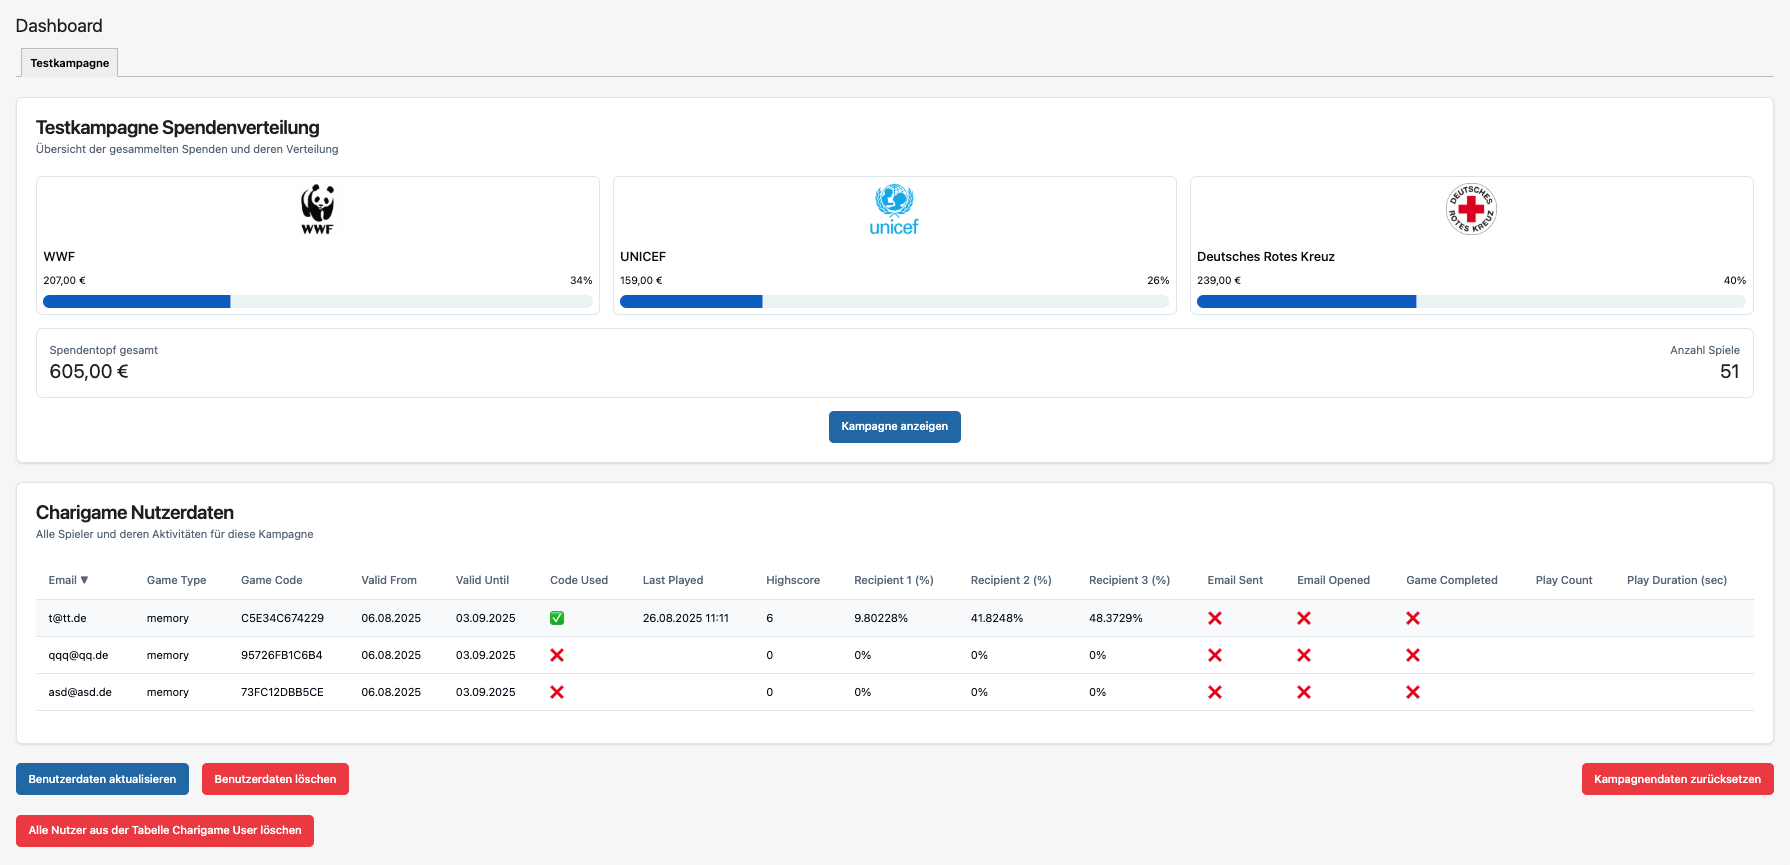
\includegraphics[width=1\textwidth]{images/new_dashboard_backend}
    \caption{Das neu aufgebaute Dashboard im Backend (eigene Darstellung)}
    \label{fig:new-dashboard-backend}
\end{figure}

\\\\
\textbf{E-Mail-Template System}

Ein umfassendes E-Mail-Template-System wurde implementiert, das HTML-Templates als Custom Post Type im Block-Editor verfügbar macht.
Dies bietet dem Redakteur die Möglichkeit, dass der Nutzer das Template der Einladungs-Mail direkt im Live-Editor anpassen kann.
Die Backendansicht des neuen Template-Systems ist folgend in Abbildung X dargestellt:

\begin{figure}[H]
    \centering
    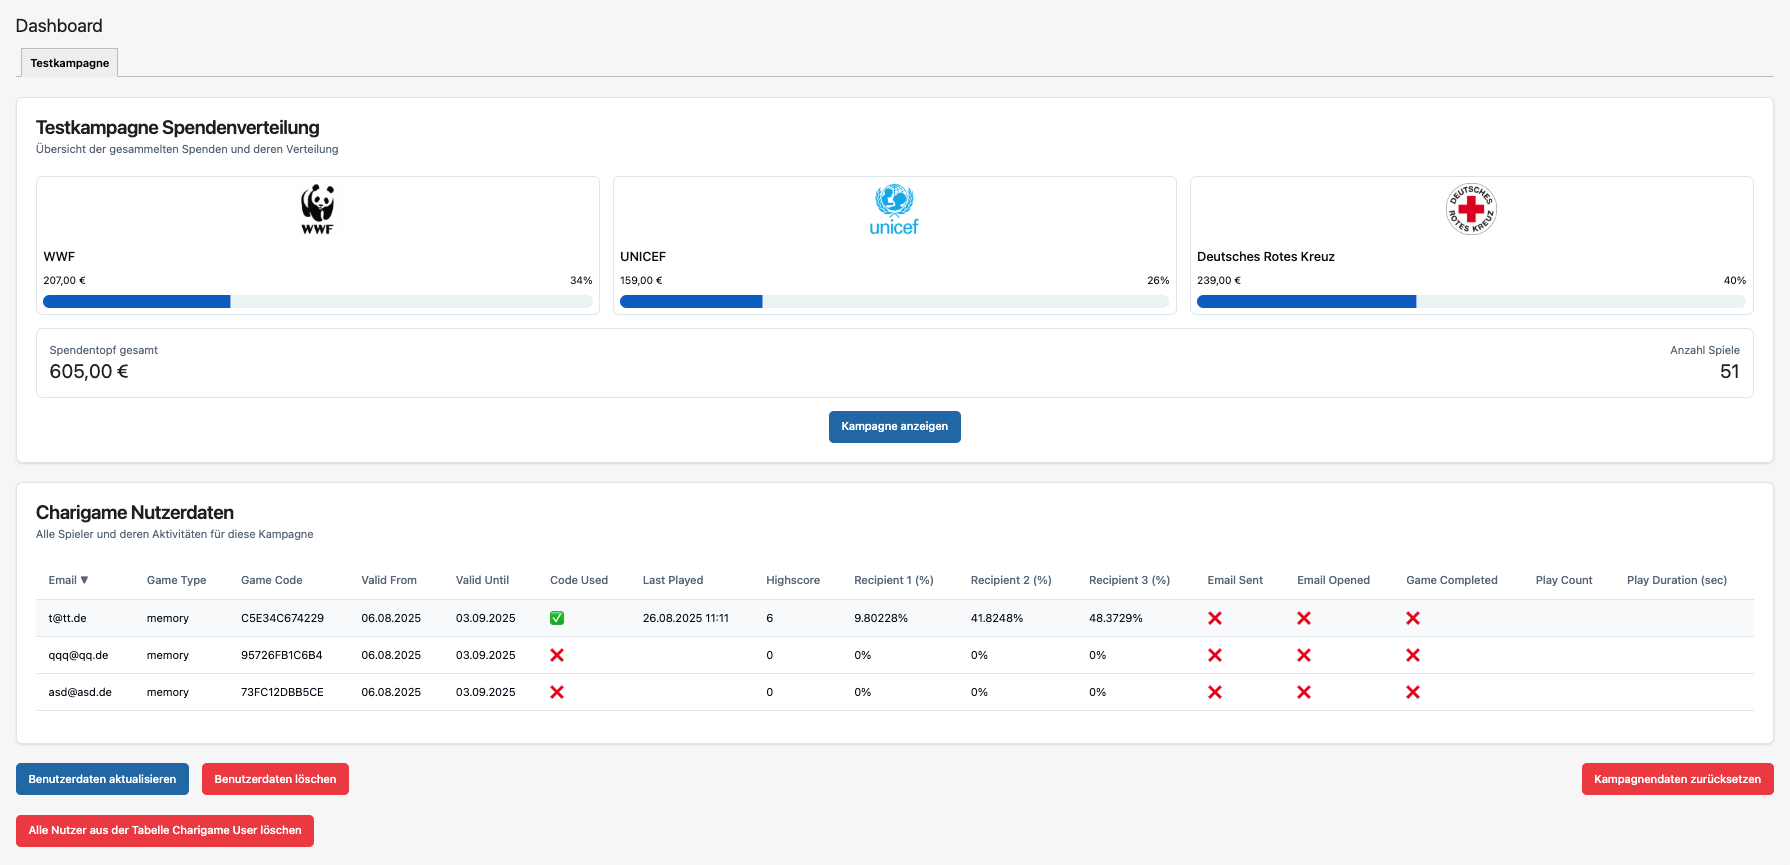
\includegraphics[width=1\textwidth]{images/new_dashboard_backend}
    \caption{Das neu aufgebaute Dashboard im Backend (eigene Darstellung)}
    \label{fig:new-dashboard-backend}
\end{figure}

Die SMTP-Konfiguration nutzt ebenfalls die erstellten shadcn-Komponenten und somit ist eine einheitliche UX gegeben %TODO: ABBILDUNG X
\\\\
\textbf{Helper Funktionen}

Während der Implementation wurden kontinuierlich verschiedene Getter- und Setter-Funktionen für die Plugin-Komponenten, AJAX-Action-Registrierung für die Frontend-Backend-Kommunikation benötigt.
Damit diese zentral und über die verschiedenen Klassen hinaus im Projekt nutzbar sind, wurde die \texttt{helper.php}-Datei als Schnittstelle//SCHNITTSTELLE VLLT NICHT DAS BESTE WORT// erstellt.
Dies bietet im Projekt eine konsistente Schnittstelle für Datenabruf und -manipulation sowie Cache-Management für Performance-Optimierung.
Als wichtige Funktionen sind u.a. ...
\\\\
\textbf{Spielintegration und Einstellungen}

Die bestehenden Spiele wurden in die neue Architektur übernommen und an die eingesetzten Bibliotheken wie Carbon Fields gemünzt.
Eine wesentliche Weiterentwicklung ist die möglichkeit individuelle Einstellungsmöglichkeiten separat zu erstellen und zu verwalten.
Das Settings-System wurde aus der Kampagne ausgelagert, um eine flexiblere Konfiguration und bessere Wartbarkeit zu gewährleisten.
Durch das Auslagern besteht nun die Möglichkeit, die hinterlegten Spieleinstellungen mehreren Kampagnen zuzuordnen.
Der entwickelte Gutenberg-Block für die Game-Section ermöglicht die dynamische Einbindung verschiedener Spieltypen über ein Template-basiertes System, das in src/games/ organisiert ist.
\\\\
\textbf{Qualitätssicherung und Standards}

Während der gesamten Implementierung wurden WordPress-Best-Practices befolgt.
Die PHPCS-Integration hat für die automatisierte Code-Standards-Prüfung gesorgt.
Es wurden stets Nonce-Validierung angewendet, welche alle AJAX-Requests schützen, Input-Sanitizing sowie Output-Escaping umgesetzt.
Außerdem ist durch die objektorientierte Programmierung mit klarer Verantwortungstrennung und Modularität für bessere Testbarkeit und Wartung gesorgt.

\section{Gutenberg-Block-Entwicklung}

Ein Kernbereich der Implementierung war der Aufbau der Gutenberg-Blöcke (\gls{blockeditor}).
Die Registrierung erfolgt im Projekt automatisiert über die Hauptklasse \texttt{ChariGame\_Blocks}, die alle Blöcke in src/blocks/ mit vorhandener \texttt{block.json} registriert (vgl. Abbildung X). %Abbildung hinterlegen
Für das \textit{ChariGame} Plugin wurde ein Block-Whitelisting implementiert, das nur die plugin-eigenen Blöcke zulässt.
Dies gewährleistet eine konsistente Benutzererfahrung und verhindert Layout-Inkonsistenzen.
Die gesamte Landingpage wie sie im Backend von den Redakteuren verwendet werden kann ist in Abbildung XY im Anhang zu erkennen. %ToDo abbildung

Die implementierten Blöcke spiegeln den Stand der Weiterentwicklung wider und sind vollständig über den Gutenberg-Editor anpassbar:

\begin{itemize}
    \item \textbf{Intro Section}: Hero-Bereich mit konfigurierbaren Farben und Typografien
    \item \textbf{Donation Section}: Dynamische Spendenverteilungs-Visualisierung
    \item \textbf{How-to-Play Section}: Spielanleitung mit HeroIcons Integration
    \item \textbf{Recipient Section}: Darstellung der Spendenempfänger
    \item \textbf{Game Section}: Templatebasierte Spielintegration
\end{itemize}

Jeder Block implementiert serverseitiges Rendering über die zugehörigen \texttt{render.php} Dateien des Blocks, um dynamische Inhalte und bessere Performance zu gewährleisten.
Zur Unterstützung der Block-Entwicklung wurden verschiedene Utilities entwickelt, damit Codedoppelungen vermieden werden.


//Auflistung der Utilities

Die colorpalette stellt ein einheitliches Farbauswahl-Interface bereit, iconlist integriert Heroicons mit SVG-Inline-Rendering, useimage behandelt Medien-Handling für Block-Attribute und usecampaigndata ermöglicht Kampagnendaten-Integration für dynamische Blöcke.

Ferner wurden Komponenten wie BackgroundSelect und BorderStyle ausgelagert, um Konstanten zentral abrufen zu können.
Während der Implementierung wurde festgestellt, dass die bestehende Spendenverteilungs-Logik nicht mehr funktionierte.
Ein neuer Donation Manager wurde entwickelt, der Kampagnen-Statistiken berechnet und cached.
Die Spendenverteilung wird nach konfigurierbaren Regeln durchführt.
Zusätzlich sind Echtzeit-Updates für die Donation Section bereitstellt und Rundungs- und Formatierungslogik implementiert.

Die Implementierung adressiert die definierten Anforderungen und schafft eine solide Basis für zukünftige Erweiterungen, welche im abschließenden Kapitel \ref{ch:fazit-und-ausblick} der Arbeit thematisiert werden.
